% answers.tex —— 2003 年·春季北京卷·理科 · 参考答案与详细解析片段
% 由 tools/generate_projects.py 依来源总账自 2003/2003_数学真题_春季北京理_试题.md + 2003/2003_数学真题_春季北京理_解析正文.md + 2003/2003_数学真题_春季北京理_答案要点.md 生成，勿手改（改源 MD 后重跑）


\begin{gktip}
项目独立求解，非官方；第8、14题待核。
\end{gktip}

\begin{answer}
\gksolhead{1}{}

\textbf{题目}：

若集合 $M=\{y\mid y=2^{-x}\}$，$P=\{y\mid y=\sqrt{x-1}\}$，则 $M\cap P=$（ ）

   (A) $\{y\mid y>1\}$　(B) $\{y\mid y\ge1\}$　(C) $\{y\mid y>0\}$　(D) $\{y\mid y\ge0\}$

\Needspace{4\baselineskip}
\textbf{解析}

$M=(0,+\infty)$，$P=[0,+\infty)$，交集 $(0,+\infty)$，选 C。

\gkanswer{答案：C。}

\end{answer}
\begin{answer}
\gksolhead{2}{}

\textbf{题目}：

若 $f(x)=\dfrac{x-1}{x}$，则方程 $f(4x)=x$ 的根是（ ）

   (A) $\frac12$　(B) $-\frac12$　(C) $2$　(D) $-2$

\Needspace{4\baselineskip}
\textbf{解析}

$x\ne0$，$(4x-1)/(4x)=x$ 化为 $(2x-1)^2=0$，$x=1/2$，选 A。

\gkanswer{答案：A。}

\end{answer}
\begin{answer}
\gksolhead{3}{}

\textbf{题目}：

设复数 $z_1=-1+i$，$z_2=\frac12+\frac{\sqrt3}{2}i$，则 $\arg\dfrac{z_1}{z_2}=$（ ）

   (A) $\frac{13}{12}\pi$　(B) $\frac7{12}\pi$　(C) $\frac5{12}\pi$　(D) $-\frac5{12}\pi$

\Needspace{4\baselineskip}
\textbf{解析}

$\arg z_1=3\pi/4$，$\arg z_2=\pi/3$，商的辐角主值 $5\pi/12$，选 C。

\gkanswer{答案：C。}

\end{answer}
\begin{answer}
\gksolhead{4}{}

\textbf{题目}：

函数 $f(x)=\dfrac1{1-x(1-x)}$ 的最大值是（ ）

   (A) $\frac45$　(B) $\frac54$　(C) $\frac34$　(D) $\frac43$

\Needspace{4\baselineskip}
\textbf{解析}

$1-x(1-x)=(x-1/2)^2+3/4$，最大值 $4/3$，选 D。

\gkanswer{答案：D。}

\end{answer}
\begin{answer}
\gksolhead{5}{}

\textbf{题目}：

在同一坐标系中，方程 $a^2x^2+b^2y^2=1$ 与 $ax+by^2=0$（$a>b>0$）的曲线大致是（ ）
\nopagebreak[4]
\begin{center}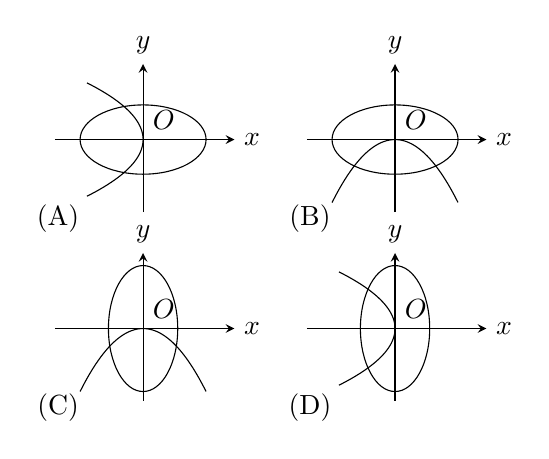
\begin{tikzpicture}[scale=.8,>=stealth]
\foreach \x/\y/\kind/\lab in {0/0/a/A,4/0/b/B,0/-3/c/C,4/-3/d/D}{
\begin{scope}[shift={(\x,\y)}]
\draw[->] (-1.4,0)--(1.45,0) node[right] {$x$}; \draw[->] (0,-1.15)--(0,1.2) node[above] {$y$};
\if\kind a \draw (0,0) ellipse (1 and .55); \draw[domain=-.9:.9,samples=50] plot ({-1.1*\x*\x},{\x});\fi
\if\kind b \draw (0,0) ellipse (1 and .55); \draw[domain=-1:1,samples=50] plot ({\x},{-\x*\x});\fi
\if\kind c \draw (0,0) ellipse (.55 and 1); \draw[domain=-1:1,samples=50] plot ({\x},{-\x*\x});\fi
\if\kind d \draw (0,0) ellipse (.55 and 1); \draw[domain=-.9:.9,samples=50] plot ({-1.1*\x*\x},{\x});\fi
\node[above right] at (0,0) {$O$}; \node at (-1.35,-1.25) {(\lab)};
\end{scope}}
\end{tikzpicture}
\end{center}
\nopagebreak[4]
\Needspace{4\baselineskip}
\textbf{解析}

椭圆横半轴 $1/a$ 小于纵半轴 $1/b$；$x=-by^2/a$ 是左开口抛物线，选 D。须在绘图时再次对照选项图。

\gkanswer{答案：D。}

\end{answer}
\begin{answer}
\gksolhead{6}{}

\textbf{题目}：

若 $A,B,C$ 是 $\triangle ABC$ 的三个内角，且 $A<B<C$（$C\ne\frac\pi2$），则下列结论中正确的是（ ）

   (A) $\sin A<\sin C$　(B) $\cos A<\cos C$　(C) $\tan A<\tan C$　(D) $\cot A<\cot C$

\Needspace{4\baselineskip}
\textbf{解析}

$A<C$ 且 $A+C=\pi-B<\pi$，因此 $\sin C-\sin A=2\cos((A+C)/2)\sin((C-A)/2)>0$，选 A。余切在 $(0,\pi)$ 严格递减，故 D 不成立。

\gkanswer{答案：A。}

\end{answer}
\begin{answer}
\gksolhead{7}{}

\textbf{题目}：

椭圆 $\begin{cases}x=4+5\cos\varphi,\\y=3\sin\varphi,\end{cases}$（$\varphi$ 为参数）的焦点坐标为（ ）

   (A) $(0,0),(0,-8)$　(B) $(0,0),(-8,0)$　(C) $(0,0),(0,8)$　(D) $(0,0),(8,0)$

\Needspace{4\baselineskip}
\textbf{解析}

椭圆中心 $(4,0)$，半焦距 $\sqrt{25-9}=4$，焦点 $(0,0),(8,0)$，选 D。

\gkanswer{答案：D。}

\end{answer}
\begin{answer}
\gksolhead{8}{}

\textbf{题目}：

如图，在正三角形 $ABC$ 中，$D,E,F$ 分别为各边的中点，$G,H,I,J$ 分别为 $AF,AD,BE,DE$ 的中点。将 $\triangle ABC$ 沿 $DE,EF,DF$ 折成三棱锥以后，$GH$ 与 $IJ$ 所成角的度数为（ ）
\nopagebreak[4]
\begin{center}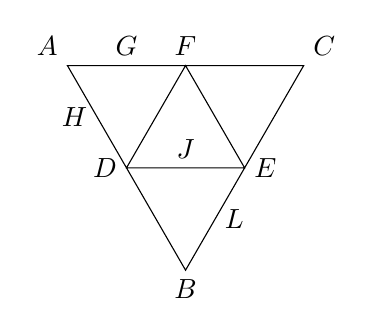
\begin{tikzpicture}[scale=1.5]
\coordinate (A) at (0,1.732); \coordinate (B) at (1,0); \coordinate (C) at (2,1.732); \coordinate (D) at (.5,.866); \coordinate (E) at (1.5,.866); \coordinate (F) at (1,1.732); \coordinate (G) at (.5,1.732); \coordinate (H) at (.25,1.299); \coordinate (I) at (1.25,.433); \coordinate (J) at (1,.866);
\draw (A)--(B)--(C)--cycle (D)--(E)--(F)--cycle;
\node[above left] at (A) {$A$}; \node[below] at (B) {$B$}; \node[above right] at (C) {$C$}; \node[left] at (D) {$D$}; \node[right] at (E) {$E$}; \node[above] at (F) {$F$}; \node[above] at (G) {$G$}; \node[left] at (H) {$H$}; \node[right] at (I) {$L$}; \node[above] at (J) {$J$};
\end{tikzpicture}
\end{center}
\nopagebreak[4]
   (A) $90^\circ$　(B) $60^\circ$　(C) $45^\circ$　(D) $0^\circ$

\Needspace{4\baselineskip}
\textbf{解析}

$GH\parallel FD$，$IJ\parallel BD$。由正三角形四等分的展开图折成正四面体，相应棱 $FD,BD$ 位于同一正三角形面，相交角为 $60^\circ$，选 B。题干 I 与图上似 L 的差异须保留，以上取题干所述 $I$ 为 $BE$ 中点。

\gkanswer{答案：U/PENDING；题干 I 为 BE 中点时选 B，图标 L 与题干不一致。}

\end{answer}
\begin{answer}
\gksolhead{9}{}

\textbf{题目}：

某班新年联欢会原定的 5 个节目已排成节目单，开演前又增加了两个新节目。如果将这两个节目插入原节目单中，那么不同插法的种数为（ ）

   (A) 42　(B) 30　(C) 20　(D) 12

\Needspace{4\baselineskip}
\textbf{解析}

两个不同新增节目依次插入原节目单的 6、7 个位置，共 $6\times7=42$，选 A。

\gkanswer{答案：A。}

\end{answer}
\begin{answer}
\gksolhead{10}{}

\textbf{题目}：

已知直线 $ax+by+c=0$（$abc\ne0$）与圆 $x^2+y^2=1$ 相切，则三条边长分别为 $|a|,|b|,|c|$ 的三角形（ ）

    (A) 是锐角三角形　(B) 是直角三角形　(C) 是钝角三角形　(D) 不存在

\Needspace{4\baselineskip}
\textbf{解析}

相切给出 $|c|/\sqrt{a^2+b^2}=1$，故 $c^2=a^2+b^2$；$a,b\ne0$，三边构成直角三角形，选 B。

\gkanswer{答案：B。}

\end{answer}
\begin{answer}
\gksolhead{11}{}

\textbf{题目}：

若不等式 $|ax+2|<6$ 的解集为 $(-1,2)$，则实数 $a$ 等于（ ）

    (A) 8　(B) 2　(C) $-4$　(D) $-8$

\Needspace{4\baselineskip}
\textbf{解析}

因解集端点是 $-1,2$，区间中心 $-2/a=1/2$，得 $a=-4$；代入验证区间，选 C。

\gkanswer{答案：C。}

\end{answer}
\begin{answer}
\gksolhead{12}{}

\textbf{题目}：

在直角坐标系 $xOy$ 中，已知 $\triangle AOB$ 三边所在直线的方程分别为 $x=0,y=0,2x+3y=30$，则 $\triangle AOB$ 内部和边上整点（即横、纵坐标均为整数的点）的总数是（ ）

    (A) 95　(B) 91　(C) 88　(D) 75

\Needspace{4\baselineskip}
\textbf{解析}

$x=0,\ldots,15$ 时，$y=0,\ldots,\lfloor(30-2x)/3\rfloor$；逐列求和 $\sum_{x=0}^{15}(\lfloor(30-2x)/3\rfloor+1)=91$，选 B。

\gkanswer{答案：B。}

\end{answer}
\begin{answer}
\gksolhead{13}{}

\textbf{题目}：

如图，一个底面半径为 $R$ 的圆柱形量杯中装有适量的水。若放入一个半径为 $r$ 的实心铁球，水面高度恰好升高 $r$，则 $\dfrac Rr=$ \gkblank{}。
\nopagebreak[4]
\begin{center}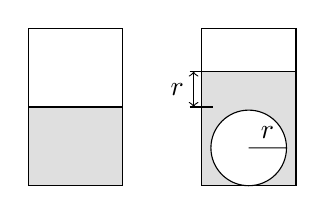
\begin{tikzpicture}[scale=1]
\fill[gray!25] (0,0) rectangle (1.2,1); \draw (0,2)--(0,0)--(1.2,0)--(1.2,2)--(0,2) (0,1)--(1.2,1);
\begin{scope}[xshift=2.2cm] \fill[gray!25] (0,0) rectangle (1.2,1.45); \draw (0,2)--(0,0)--(1.2,0)--(1.2,2)--(0,2); \draw (0,1.45)--(1.2,1.45); \fill[white] (.6,.48) circle (.48); \draw (.6,.48) circle (.48) (.6,.48)--(1.08,.48) node[midway,above] {$r$}; \draw (-.15,1)--(.15,1) (-.15,1.45)--(.15,1.45); \draw[<->] (-.1,1)--(-.1,1.45) node[midway,left] {$r$}; \end{scope}
\end{tikzpicture}
\end{center}
\nopagebreak[4]
\Needspace{4\baselineskip}
\textbf{解析}

图中铁球完全浸没，排水体积 $\pi R^2r=4\pi r^3/3$，所以 $R/r=2/\sqrt3$。

\gkanswer{答案：$2/\sqrt3$。}

\end{answer}
\begin{answer}
\gksolhead{14}{}

\textbf{题目}：

在某报《自测健康状况》的报道中，自测血压结果与相应年龄的统计数据如下表。观察表中数据的特点，用适当的数填入表中空白内。

\begin{center}
\begingroup\setlength{\tabcolsep}{4pt}
\begin{tabular}{lllllllll}
\toprule
年龄（岁） & 30 & 35 & 40 & 45 & 50 & 55 & 60 & 65 \\
\midrule
收缩压（水银柱/毫米） & 110 & 115 & 120 & 125 & 130 & 135 &  & 145 \\
舒张压（水银柱/毫米） & 70 & 73 & 75 & 78 & 80 & 83 &  & 88 \\
\bottomrule
\end{tabular}
\endgroup
\end{center}

\Needspace{4\baselineskip}
\textbf{解析}

收缩压每 5 岁加 5，60 岁为 140；舒张压每 10 岁加 5，60 岁为 85。这只是符合所示数据的一种常见规律，有限数据不能唯一确定缺失值，须标记为推测并待其他来源核实。

\gkanswer{答案：U/PENDING；140、85 仅为一种可能规律。}

\end{answer}
\begin{answer}
\gksolhead{15}{}

\textbf{题目}：

已知 $F_1,F_2$ 分别为椭圆 $\dfrac{x^2}{a^2}+\dfrac{y^2}{b^2}=1$ 的左、右焦点，点 $P$ 在椭圆上，$\triangle POF_2$ 是面积为 $\sqrt3$ 的正三角形，则 $b^2$ 的值是 \gkblank{}。

\Needspace{4\baselineskip}
\textbf{解析}

正三角形面积 $\sqrt3$，边长 $2$，所以 $OF_2=2$，焦距参数 $c=2$。设 $P=(1,\pm\sqrt3)$，则 $PF_2=2$，$PF_1=2\sqrt3$，$2a=2+2\sqrt3$，故 $b^2=a^2-c^2=2\sqrt3$。

\gkanswer{答案：$2\sqrt3$。}

\end{answer}
\begin{answer}
\gksolhead{16}{}

\textbf{题目}：

若存在常数 $p>0$，使得函数 $f(x)$ 满足 $f(px)=f(px-\dfrac p2)$（$x\in\mathbb R$），则 $f(x)$ 的一个正周期为 \gkblank{}。

\Needspace{4\baselineskip}
\textbf{解析}

令 $t=px$，因 $p>0$ 有 $t$ 遍历实数，$f(t)=f(t-p/2)$，因此 $p/2$ 是一个正周期；不声称它是最小正周期。

\gkanswer{答案：$p/2$。}

\end{answer}
\begin{answer}
\gksolhead{17}{}

\textbf{题目}：

解不等式：$\log_{\frac12}(x^2-x-2)>\log_{\frac12}(x-1)-1$。

\Needspace{4\baselineskip}
\textbf{解析}

对数真数均正，得 $x>2$。底数 $1/2<1$，且 $\log_{1/2}(x-1)-1=\log_{1/2}(2x-2)$，故 $x^2-x-2<2x-2$，即 $x(x-3)<0$。结合定义域得 $(2,3)$。

\gkanswer{答案：$(2,3)$。}

\end{answer}
\begin{answer}
\gksolhead{18}{}

\textbf{题目}：

已知函数 $f(x)=\dfrac{6\cos^4x+5\sin^2x-4}{\cos2x}$，求 $f(x)$ 的定义域，判断它的奇偶性，并求其值域。

\Needspace{4\baselineskip}
\textbf{解析}

设 $t=\cos2x$，$t\in[-1,1]\setminus\{0\}$。代入 $\cos^2x=(1+t)/2$、$\sin^2x=(1-t)/2$，分子为 $(3t^2+t)/2$，故 $f=3t/2+1/2$。定义域为 $\mathbb R\setminus\{\pi/4+k\pi/2:k\in\mathbb Z\}$，函数为偶函数，值域为 $[-1,1/2)\cup(1/2,2]$。

\gkanswer{答案：定义域 $\mathbb R\setminus\{\pi/4+k\pi/2:k\in\mathbb Z\}$；偶函数；值域 $[-1,1/2)\cup(1/2,2]$。}

\end{answer}
\begin{answer}
\gksolhead{19}{}

\textbf{题目}：

如图，正四棱柱 $ABCD-A_1B_1C_1D_1$ 中，底面边长为 $2\sqrt2$，侧棱长为 $4$。$E,F$ 分别为棱 $AB,BC$ 的中点，$EF\cap BD=G$。

（1） 求证：平面 $B_1EF\perp$ 平面 $BDD_1B_1$；

（2） 求点 $D_1$ 到平面 $B_1EF$ 的距离 $d$；

（3） 求三棱锥 $B_1-EFD_1$ 的体积 $V$。
\nopagebreak[4]
\begin{center}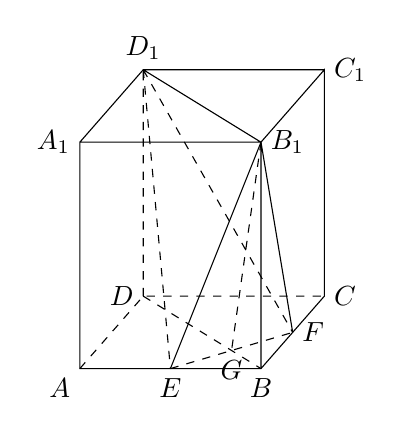
\begin{tikzpicture}[scale=1.15]
\coordinate (A) at (0,0); \coordinate (B) at (2,0); \coordinate (C) at (2.7,.8); \coordinate (D) at (.7,.8); \coordinate (Ap) at (0,2.5); \coordinate (Bp) at (2,2.5); \coordinate (Cp) at (2.7,3.3); \coordinate (Dp) at (.7,3.3); \coordinate (E) at (1,0); \coordinate (F) at (2.35,.4); \coordinate (G) at (1.675,.2);
\draw (A)--(B)--(C)--(Cp)--(Bp)--(Ap)--cycle (Ap)--(Dp)--(Cp) (Dp)--(Bp) (Bp)--(B) (E)--(Bp) (F)--(Bp);
\draw[dashed] (A)--(D)--(C) (D)--(Dp) (D)--(B) (E)--(F) (Bp)--(G) (Dp)--(E) (Dp)--(F);
\foreach \p/\place/\lab in {A/below left/A,B/below/B,C/right/C,D/left/D,E/below/E,F/right/F,G/below/G,Ap/left/{A_1},Bp/right/{B_1},Cp/right/{C_1},Dp/above/{D_1}} \node[\place] at (\p) {$\lab$};
\end{tikzpicture}
\end{center}
\nopagebreak[4]
\Needspace{4\baselineskip}
\textbf{解析}

\gksubpart{(1)}

取 $B=(0,0,0),A=(2\sqrt2,0,0),C=(0,2\sqrt2,0),D=(2\sqrt2,2\sqrt2,0),B_1=(0,0,4)$，则 $E=(\sqrt2,0,0),F=(0,\sqrt2,0),D_1=(2\sqrt2,2\sqrt2,4)$。平面 $B_1EF$ 方程 $x+y+z/(2\sqrt2)=\sqrt2$；平面 $BDD_1B_1$ 方程 $x-y=0$，法向量内积为零，证明垂直。

\gksubpart{(2)}

$D_1$ 到前一平面距离为 $4\sqrt2/\sqrt{17/8}=16/\sqrt{17}=16\sqrt{17}/17$。

\gksubpart{(3)}

以 $B_1$ 为共同顶点，三棱锥体积 $|\det(E-B_1,F-B_1,D_1-B_1)|/6=32/6=16/3$。

\gkanswer{答案（1）：证明见解析。}

\gkanswer{答案（2）：$16/\sqrt{17}$。}

\gkanswer{答案（3）：$16/3$。}

\end{answer}
\begin{answer}
\gksolhead{20}{}

\textbf{题目}：

某租赁公司拥有汽车 100 辆。当每辆车的月租金为 3000 元时，可全部租出。当每辆车的月租金每增加 50 元时，未租出的车将会增加一辆。租出的车每辆每月需要维护费 150 元，未租出的车每辆每月需要维护费 50 元。

（1） 当每辆车的月租金定为 3600 元时，能租出多少辆车？

（2） 当每辆车的月租金定为多少元时，租赁公司的月收益最大？最大月收益是多少？

\Needspace{4\baselineskip}
\textbf{解析}

\gksubpart{(1)}

月租增加 $k$ 次 50 元，租出 $100-k$ 辆。收益 $R=(3000+50k)(100-k)-150(100-k)-50k=285000+2100k-50k^2$。 租金 3600 元时 $k=12$，租出 88 辆；

\gksubpart{(2)}

抛物线顶点 $k=21$ 属可行整数，租金 4050 元，最大月收益 307050 元。

\gkanswer{答案（1）：88 辆。}

\gkanswer{答案（2）：月租 4050 元；最大月收益 307050 元。}

\end{answer}
\begin{answer}
\gksolhead{21}{}

\textbf{题目}：

如图，在边长为 $l$ 的等边 $\triangle ABC$ 中，圆 $O_1$ 为 $\triangle ABC$ 的内切圆，圆 $O_2$ 与圆 $O_1$ 外切，且与 $AB,BC$ 相切，$\cdots$，圆 $O_{n+1}$ 与圆 $O_n$ 外切，且与 $AB,BC$ 相切，如此无限继续下去。记圆 $O_n$ 的面积为 $a_n$（$n\in\mathbb N$）。

（1） 证明 $\{a_n\}$ 是等比数列；

（2） 求 $\lim_{n\to\infty}(a_1+a_2+\cdots+a_n)$ 的值。
\nopagebreak[4]
\begin{center}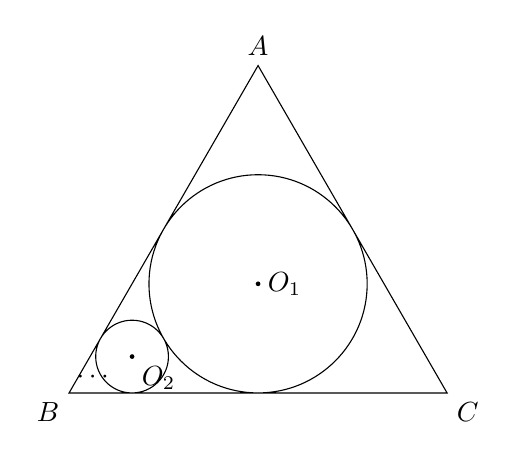
\begin{tikzpicture}[scale=1.2]
\coordinate (B) at (0,0); \coordinate (C) at (4,0); \coordinate (A) at (2,3.464); \coordinate (Oone) at (2,1.1547); \coordinate (Otwo) at (.6667,.3849);
\draw (A)--(B)--(C)--cycle (Oone) circle (1.1547) (Otwo) circle (.3849);
\fill (Oone) circle (.025) (Otwo) circle (.025); \node[right] at (Oone) {$O_1$}; \node[below right] at (Otwo) {$O_2$}; \node[above] at (A) {$A$}; \node[below left] at (B) {$B$}; \node[below right] at (C) {$C$}; \node at (.25,.16) {$\cdots$};
\end{tikzpicture}
\end{center}
\nopagebreak[4]
\Needspace{4\baselineskip}
\textbf{解析}

\gksubpart{(1)}

$\angle B=60^\circ$，圆心在角平分线上，距 $B$ 为半径两倍。相邻圆外切给出 $2(r_n-r_{n+1})=r_n+r_{n+1}$，所以 $r_{n+1}=r_n/3$，面积比为 $1/9$。

\gksubpart{(2)}

首圆为边长 $l$ 的正三角形内切圆，半径 $l\sqrt3/6$，$a_1=\pi l^2/12$。故面积级数和 $a_1/(1-1/9)=3\pi l^2/32$。

\gkanswer{答案（1）：证明见解析。}

\gkanswer{答案（2）：$3\pi l^2/32$。}

\end{answer}
\begin{answer}
\gksolhead{22}{}

\textbf{题目}：

已知动圆过定点 $P(1,0)$，且与定直线 $l:x=-1$ 相切，点 $C$ 在 $l$ 上。

（1） 求动圆圆心的轨迹 $M$ 的方程；

（2） 设过点 $P$，且斜率为 $-\sqrt3$ 的直线与曲线 $M$ 相交于 $A,B$ 两点。

① 问：$\triangle ABC$ 能否为正三角形？若能，求点 $C$ 的坐标；若不能，说明理由；

② 当 $\triangle ABC$ 为钝角三角形时，求这种点 $C$ 的纵坐标的取值范围。

\Needspace{4\baselineskip}
\textbf{解析}

\gksubpart{(1)}

圆心到 $P(1,0)$ 的距离等于到 $x=-1$ 的距离，得轨迹 $M:y^2=4x$。

\gksubpart{(2)}

代入 $y=-\sqrt3(x-1)$，得 $3(x-1)^2=4x$，即 $3x^2-10x+3=0$；取 $A=(3,-2\sqrt3)$，$B=(1/3,2\sqrt3/3)$。以 $AB$ 为边的等边三角形的第三顶点横坐标为 $-7/3$ 或 $17/3$，不在 $x=-1$ 上，故不能为正三角形。

\Needspace{5\baselineskip}
令 $C=(-1,t)$。三个角的相应向量点积分别为

\nopagebreak[4]
\[\overrightarrow{AB}\cdot\overrightarrow{AC}=\frac{8}{3}(10+\sqrt3 t),\quad \overrightarrow{BA}\cdot\overrightarrow{BC}=\frac{16}{9}-\frac{8\sqrt3}{3}t,\quad \overrightarrow{CA}\cdot\overrightarrow{CB}=\left(t+\frac{2\sqrt3}{3}\right)^2.\]

故 $A$ 为钝角当且仅当 $t<-10/\sqrt3$，$B$ 为钝角当且仅当 $t>2/(3\sqrt3)$，$C$ 不可能为钝角。还须排除 $t=2\sqrt3$，因为此时 $C$ 位于直线 $AB$ 上，三点共线。故所求为 $(-\infty,-10/\sqrt3)\cup(2/(3\sqrt3),2\sqrt3)\cup(2\sqrt3,+\infty)$。

\gkanswer{答案（1）：$y^2=4x$。}

\gkanswer{答案（2）：不能为正三角形；钝角时 $t\in(-\infty,-10/\sqrt3)\cup(2/(3\sqrt3),2\sqrt3)\cup(2\sqrt3,+\infty)$。}

\end{answer}